\documentclass[]{article}

% Imported Packages
%------------------------------------------------------------------------------
\usepackage{amssymb}
\usepackage{amstext}
\usepackage{amsthm}
\usepackage{amsmath}
\usepackage{enumerate}
\usepackage{fancyhdr}
\usepackage[margin=1in]{geometry}
\usepackage{graphicx}
\usepackage{extarrows}
\usepackage{setspace}
\usepackage{float}
%------------------------------------------------------------------------------

% Header and Footer
%------------------------------------------------------------------------------
\pagestyle{plain}
\renewcommand\headrulewidth{0.4pt}
\renewcommand\footrulewidth{0.4pt}
%------------------------------------------------------------------------------

% Title Details
%------------------------------------------------------------------------------
\title{
  Erudite\\
  \large \emph{An educational content management system}\\
  \vspace{1em}
  High-Level Architectural Design
}
\author{
  SE 3A04: Software Design II -- Large System Design
  \\
  \begin{tabular}{ l l }
    Kelvin Lin*   & STUDENT-NUM \\
    Danish Khan   & STUDENT-NUM \\
    Puru Jetly    & STUDENT-NUM \\
    Terrance Yip  & STUDENT-NUM \\
    Varun Hooda   & STUDENT-NUM \\
  \end{tabular}
}
\date{}
%------------------------------------------------------------------------------

% Document
%------------------------------------------------------------------------------
\begin{document}

\maketitle
\newpage

\tableofcontents
\newpage

\section{Introduction}
\label{sec:introduction}
This section outlines the purpose and provides a system description of the
Erudite project; along with an overview of the contents and organization of
this high-level architectural design document.


\subsection{Purpose}
\label{sub:purpose}
The purpose of this document to define the use cases, layout the Analysis Class
Diagram, describe the Architectural Design, and finally document the class
responsibilities through collaboration cards. This document builds on top of
and extends the Software Requirements Specification document in that this
document describes the way in which the system will interact with the outside
world and how the subsystems will be architecturally and logically arranged.

The target audience for this document are the stakeholders (Dr. Ridha Khedri,
Andrew Le Clair and Michael Liut), and any current or future architects,
designers and developers of this project.


\subsection{System Description}
\label{sub:system_description}
The Erudite application is intended to be an educational content management
system for use in elementary school classrooms. The primary interface between
the user and the software system is through a device running the Android
operating system. This document defines the way in which the users will be
expected to interact with the system and how the application will be decomposed
into smaller subsystems to reduce the complexity and improve the
maintainability, flexibility of this system.

Specifically, the users of this system (application) are expected to perform a
set of events that will prompt the system to react. The decomposition will then
show how the subsystems will communicate among one another in order to
efficiently distribute the work and perform the required actions in response to
the user's actions.


\subsection{Overview}
\label{sub:overview}
The remainder of the document is organized into 4 sections: Use Case Diagram --
how the users and system will interact, Analysis Class Diagram -- the
subsystems that compose this entire application, Architectural Design -- the
layout of the subsystems into a well-understood software architecture, and
Class responsibility collaboration Cards -- description of the interactions
between the subsystems. Each section uses an appropriate notation and diagrams
to document the design decision and describe the details of the high-level
design of this system.


% End Section


\newpage

\section{Use Case Diagram}
\label{sec:use_case_diagram}
% Begin Section
The following diagram is an use case diagram for Erudite.\\

{
  \centering
  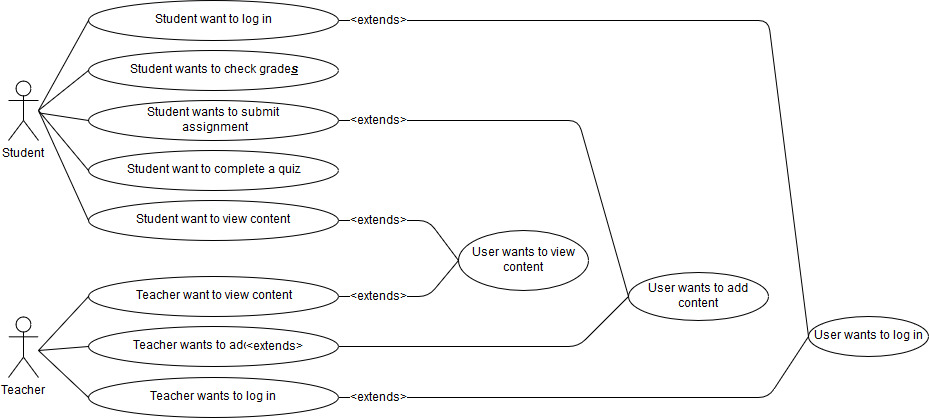
\includegraphics[scale=0.40]{A2_Assets/Use_Case_Diagram_v1.jpg}
}

\newpage

\section{Analysis Class Diagram}
\label{sec:analysis_class_diagram}
% Begin Section
The following diagram is an analysis class diagram for Erudite.\\

{
  \centering
  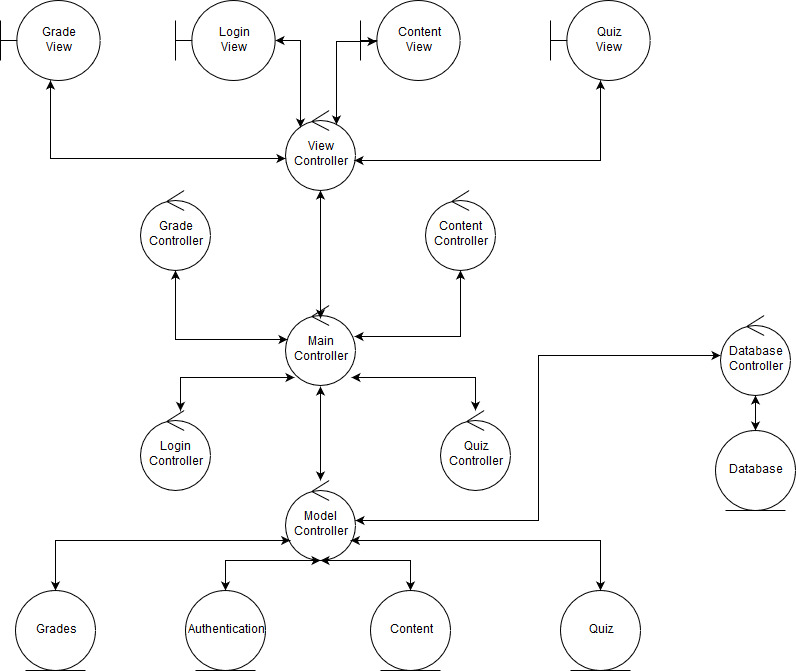
\includegraphics[scale=0.5]{A2_Assets/Analysis_Class_Diagrm_v2.jpg}
}


\section{Architectural Design}
\label{sec:architectural_design}
% Begin Section




\subsection{System Architecture}
\label{sub:system_architecture}
% Begin SubSection
Erudite will be built following the PAC architecture, where the system will be decomposed into a hierarchy of control modules, abstraction modules, and presentation modules.

The PAC architecture was chosen because Erudite is composed with multiple subsystems with interactive requirements. Each subsystem requires a view to display information, data which it processes for different users, and a controller to determine the sequence of events.

The main advantages of choosing the PAC architecture is it separates the different subsystems, and this allows for different people to implement the different subsystems independently of each other. Moreover, each component of the subsystem can also be separated so that each component can be implemented independently of each other.

Furthermore, the PAC architecture allows for high cohesion and low coupling systems. Each subsystem only interacts with the main controller, and all of the components of the subsystem are needed in order for the subsystem to fulfil its function.


%Add a structural architecture diagram here
{
  \centering
    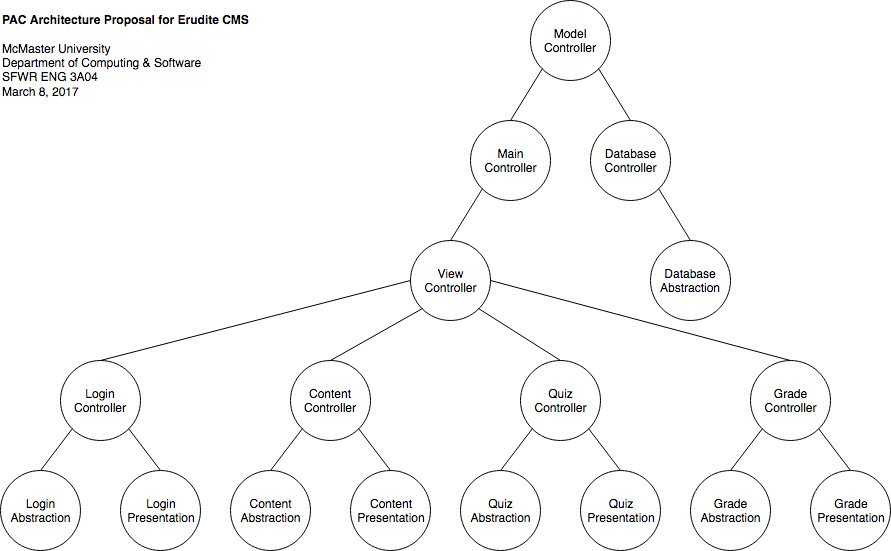
\includegraphics[scale=0.5]{A2_Assets/Structural_Class_Diagram_v2.jpg}
  \centerline{Structural Class Diagram}
}
% End SubSection

\subsection{Subsystems}
\label{sub:subsystems}
% Begin SubSection
\begin{enumerate}[a)]
	\item Provide a brief description of each subsystem. Be sure to document its
purpose and relationship to other subsystems.
\end{enumerate}

\subsubsection{The Content Management System}
The content management system is responsible for receiving and displaying content to the users. It is connected to the control system which dictates when this system is active, and it sends requests to the main control to be forwarded to the model for data processing, and to the view for display.

\subsubsection{The Quiz Management System}
WRITE SOMETHING HERE

\subsubsection{The Grade Management System}
WRITE SOMETHING HERE

\subsubsection{The Authentication System}
WRITE SOMETHING HERE
% End SubSection

% End Section

\section{Class Responsibility Collaboration (CRC) Cards}
\label{sec:class_responsibility_collaboration_crc_cards}
% Begin Section
This section should contain all of your CRC cards.

\begin{enumerate}[a)]
	\item Provide a CRC Card for each identified class
	\item Please use the format outlined in tutorial, i.e.,

  \begin{table}[H]
		\centering
		\begin{tabular}{|p{9cm}|p{3cm}|}
		\hline
		 \multicolumn{2}{|l|}{\textbf{Class Name:} LoginView} \\
		\hline
		\textbf{Responsibility:} & \textbf{Collaborators:} \\
		\hline
    Handles self-render request & ViewController \\
    \hline
    Requests to render ContentView & ViewController \\
    \hline
    Requests to render GradeView & ViewController \\
    \hline
    Requests to render QuizView & ViewController \\
    \hline
    Handles keyboard input & \\
    \hline
    Send login request to ViewController & ViewController \\
    \hline
    Send username and password pair to ViewController & ViewController \\
    \hline
    Prompt user if login request fails & ViewController \\
    \hline
    Request view change & ViewController \\
    \hline
		\end{tabular}
	\end{table}

  \begin{table}[H]
		\centering
		\begin{tabular}{|p{9cm}|p{3cm}|}
		\hline
		 \multicolumn{2}{|l|}{\textbf{Class Name:} ContentView} \\
		\hline
		\textbf{Responsibility:} & \textbf{Collaborators:} \\
		\hline
    Handles self-render request & ViewController \\
    \hline
    Requests to render LoginView & ViewController \\
    \hline
    Requests to render GradeView & ViewController \\
    \hline
    Requests to render QuizView & ViewController \\
    \hline
    Handles keyboard input & \\
    \hline
    Send course-content request to ViewController & ViewController \\
    \hline
    Send specific-file request to ViewController & ViewController \\
    \hline
    Display course content list & \\
    \hline
    Display specific file content list & \\
    \hline
    Request view change & ViewController \\
    \hline
		\end{tabular}
	\end{table}

  \begin{table}[H]
    \centering
    \begin{tabular}{|p{9cm}|p{3cm}|}
    \hline
     \multicolumn{2}{|l|}{\textbf{Class Name:} GradeView} \\
    \hline
    \textbf{Responsibility:} & \textbf{Collaborators:} \\
    \hline
    Handles self-render request & ViewController \\
    \hline
    Requests to render LoginView & ViewController \\
    \hline
    Requests to render ContentView & ViewController \\
    \hline
    Requests to render QuizView & ViewController \\
    \hline
    Handles keyboard input & \\
    \hline
    Display current course grades list & \\
    \hline
    Display current cumulative grade point average list & \\
    \hline
    Request view change & ViewController \\
    \hline
    \end{tabular}
  \end{table}

  \begin{table}[H]
    \centering
    \begin{tabular}{|p{9cm}|p{3cm}|}
    \hline
     \multicolumn{2}{|l|}{\textbf{Class Name:} QuizView} \\
    \hline
    \textbf{Responsibility:} & \textbf{Collaborators:} \\
    \hline
    Handles self-render request & ViewController \\
    \hline
    Requests to render LoginView & ViewController \\
    \hline
    Requests to render ContentView & ViewController \\
    \hline
    Requests to render GradeView & ViewController \\
    \hline
    Handles keyboard input & \\
    \hline
    Request course quiz list & ViewController \\
    \hline
    Request specific quiz & ViewController \\
    \hline
    Display course quiz list & \\
    \hline
    Display selected quiz & \\
    \hline
    Handles user answer selection & \\
    \hline
    Send quiz answers & ViewController \\
    \hline
    Request view change & ViewController \\
    \hline
    \end{tabular}
  \end{table}

	%quiz controller
	\begin{table}[H]
	\centering
		\begin{tabular}{|p{5cm}|p{5cm}|}
		\hline
		 \multicolumn{2}{|l|}{\textbf{Class Name: Quiz Controller}} \\
		\hline
		\textbf{Responsibility:} & \textbf{Collaborators:} \\
		\hline
		Knows Main Controller & \\
		\hline
		Receive quiz request from Main Controller & Main Controller \\
		\hline
		Send quiz request to Main Controller & Main Controller \\
		\hline
		Receive quiz result from Main Controller & Main Controller \\
		\hline
		Process quiz result from Main Controller & Main Controller \\
		\hline
		Receive student answer from Main Controller & Main Controller \\
		\hline
		Send request for solutions to Main Controller & Main Controller \\
		\hline
		Receive solutions from Main Controller & Main Controller \\
		\hline
		Mark quiz according to solution & \\
		\hline
		Send grade of quiz to Main Controller & Main Controller \\
		\hline

		\end{tabular}
	\end{table}

	%Grade Controller

	\begin{table}[H]
	\centering
		\begin{tabular}{|p{5cm}|p{5cm}|}
		\hline
		 \multicolumn{2}{|l|}{\textbf{Class Name: Grade Controller}} \\
		\hline
		\textbf{Responsibility:} & \textbf{Collaborators:} \\
		\hline
		Know Main Controller \\
		\hline
		Receive grade request from Main Controller & Main Controller \\
		\hline
		Send grade response to Main Controller & Main Controller \\
		\hline
		Receive grades from Main Controller & Main Controller \\
		\hline
		Process grades & \\
		\hline
		Send grades to Main Controller & Main Controller \\
		\hline
		\end{tabular}
	\end{table}

		%Model Controller

	\begin{table}[H]
	\centering
		\begin{tabular}{|p{5cm}|p{5cm}|}
		\hline
		 \multicolumn{2}{|l|}{\textbf{Class Name: Model Controller}} \\
		\hline
		\textbf{Responsibility:} & \textbf{Collaborators:} \\
		\hline
		Knows Main Controller & \\
		\hline
		Knows Database Controller & \\
		\hline
		Knows Grades Entity & \\
		\hline
		Know Authentication Token Entity & \\
		\hline
		Knows Content Entity & \\
		\hline
		Knows Quiz Entity & \\
		\hline
		Receive encrypted username and password & Main Controller \\
		\hline
		Send to Database Handler & Database Controller \\
		\hline
		Receive response object from Database Handler & Database Controller \\
		\hline
		Send response object from Database and return to Main Controller & Main \\
		\hline
		Receive authentication token storage request & Main Controller \\
		\hline
		Store authentication token & Authentication Token Entity \\
		\hline
		Receive content request & Main \\
		\hline
		Get authentication token & Authentication Token Entity \\
		\hline
		Send content request and authentication token & Database Controller \\
		\hline
		Receive content response & Database Controller \\
		\hline
		Send content response & Main Controller \\
		\hline
		Receive quiz request & Main Controller \\
		\hline
		Get authentication token & Authentication Token Entity \\
		\hline
		Send quiz request and authentication token & Database Controller\\
		\hline
		Receive quiz response & Database Controller \\
		\hline
		Send quiz response & Main Controller \\
		\hline
		Receive quiz solution request & Main Controller \\
		\hline
		Get authentication token & Authentication Token Entity \\
		\hline
		Send quiz solution request and authentication token & Database Controller \\
		\hline
		Receive quiz grade response & Database Controller \\
		\hline
		Send quiz grade response & Main \\
		\hline
		Receive grades request & Main \\
		\hline
		Get authentication token & Authentication Model \\
		\hline
		Send grades request and authentication token & Database Controller \\
		\hline
		Receive grades response & Database Controller \\
		\hline
		Send grades response & Main \\
		\hline
		\end{tabular}
	\end{table}

		%Database Controller

	\begin{table}[H]
	\centering
		\begin{tabular}{|p{5cm}|p{5cm}|}
		\hline
		 \multicolumn{2}{|l|}{\textbf{Class Name: Database Controller}} \\
		\hline
		\textbf{Responsibility:} & \textbf{Collaborators:} \\
		\hline
		Knows Model Controller & \\
		\hline
		Knows Database Entity & \\
		\hline
		Receive encrypted username and password from model handler & Model Handler \\
		\hline
		Verify username and password with the database & Database \\
		\hline
		Send response object to the model handler & Model Controller \\
		\hline
		Receive content request and authentication token & Model Controller \\
		\hline
		Grab content from database & Database \\
		\hline
		Send content response & Model Controller \\
		\hline
		Receive quiz request and authentication token & Model Controller \\
		\hline
		Grab quiz from database & Database \\
		\hline
		Send quiz response & Model Controller \\
		\hline
		Receive quiz solution request and authentication token & Model 		Controller \\
		\hline
		Grab quiz solution from database & Database \\
		\hline
		Send quiz solution response & Model Controller \\
		\hline
		Receive grade update request and authentication token & Model Controller \\
		\hline
		Update grades from database & Database \\
		\hline
		Receive grade request and authentication token & Model 	Controller \\
		\hline
		Grab grades from database & Database \\
		\hline
		Send grades response & Model Controller \\
		\hline
		\end{tabular}
	\end{table}

\end{enumerate}
% End Section


\newpage
\appendix
\section{Division of Labour}
\label{sec:division_of_labour}
\begin{description}
  \item [Kelvin Lin ]
  \item{Foo}
  \hfill \rule{2in}{0.1pt}
  \\\\

  \item [Danish Khan]
  \item{CRC Cards}
  \item{Structural Class Diagram}
  \hfill \rule{2in}{0.1pt}
  \\\\

  \item [Puru Jetly]
  \item{Baz}
  \hfill \rule{2in}{0.1pt}
  \\\\

  \item [Terrance Yip]
  \item{Qux}
  \hfill \rule{2in}{0.1pt}
  \\\\

  \item [Varun Hooda]
  \item{Section 1 Introduction}
  \item{Revision to use case diagram}
  \hfill \rule{2in}{0.1pt}
  \\\\
\end{description}

\newpage
\section{Apportioning of Requirements}
The following business events will not be addressed in the future deliverables.

\begin{enumerate}[{BE}1.]
	\item A teacher wants to create a course.
	\begin{enumerate}[{VP1}.1]
		\item Student Viewpoint
			\begin{enumerate}
				\item Students shall be able to enrol in an existing course owned by the
teacher provided the course is set visible.
			\end{enumerate}
		\item Teacher Viewpoint
			\begin{enumerate}
			    \item The teacher shall own the created course.
				\item A teacher shall be able to choose to unenroll a student from a course
that the teacher owns.
				\item A teacher shall not be enrolled in a course.
			\end{enumerate}
		\item Parent Viewpoint
			\begin{enumerate}
				\item Parents shall be able to view the course's progress or student
performance through their child's account.
			\end{enumerate}
		\item School Administration Viewpoint
			\begin{enumerate}
				\item The school administration shall be allowed to choose to whether to
allow students and teachers
to create their own accounts, or create accounts for all students and teachers.
			\end{enumerate}
		\item Information Technology Team Viewpoint
			\begin{enumerate}
				\item None
			\end{enumerate}
		\item Government \& School Board Viewpoint
			\begin{enumerate}
				\item All courses, course content, student content and any teacher student
communication held on the on the system shall be made visible to the school
board.
			\end{enumerate}
	\end{enumerate}

	\item A teacher wants to add content to a course they own.
	\begin{enumerate}[{VP1}.1]
		\item Student Viewpoint
			\begin{enumerate}
        \item A student enrolled in a course shall be able to view any content within the course when the content is set visible by the owner of that course.
        \item The system shall provide interface elements that allow the student to view any content set visible by the course owner.
        \item A student shall be able to submit an \underline{assignment}; a piece of content uploaded in response to a manual-evaluational content when the manual-evaluational content is set visible by the owner of that course and file submission is enabled.
        \item The system shall provide interface elements that allow the student to submit an assignment in response to manual-evaltional content.
        \item A student shall be able to submit an automated-evaluational content when it is set visible by the owner of that course.
        \item The system shall provide interface elements that allow the student to open and submit automated-evaluational content that is set visible by the owner of the course.
			\end{enumerate}
		\item Teacher Viewpoint
			\begin{enumerate}
				\item Teachers shall be allowed to set permissions that students have over each file.
        \item The system shall provide interface elements that allow the teacher to set permissions that students have over each file.
				\item The teacher shall specify a time period for which file submission is accepted by the manual-evaluational piece of content for manual-evaluational content.
        \item The system shall provide interface elements that allow the teacher to speicify the time period for which file submission is accepted by manual-evaluational content.
			\end{enumerate}
		\item Parent Viewpoint
			\begin{enumerate}
				\item None
			\end{enumerate}
		\item School Administration Viewpoint
			\begin{enumerate}
				\item None
			\end{enumerate}
		\item Information Technology Team Viewpoint
			\begin{enumerate}
				\item None
			\end{enumerate}
		\item Government \& School Board Viewpoint
			\begin{enumerate}
				\item None
			\end{enumerate}
	\end{enumerate}

	\item A teacher wants to add automated-evaluational content.
	\begin{enumerate}[{VP2}.1]

		\item Student Viewpoint
			\begin{enumerate}
        \item Students shall be able to view the automated-evaluational content
          only if the teacher sets the visibility of the content to be viewable
          by students.

        \item Students shall be able to open automated-evaluational content for
          a predefined period of time specified by the course owner when the
          content is made visible.

        \item Automated-evaluational content that has been opened and viewed by
          a student shall be submitted manually by the student or automatically
          before or at the end of predefined time (as specified by the teacher)
          respectively.
			\end{enumerate}

		\item Teacher Viewpoint
			\begin{enumerate}
        \item The teacher shall specify the visibility of the
          automated-evaluational content or it will default to "not visible to
          students".
			\end{enumerate}

		\item Parent Viewpoint
			\begin{enumerate}
				\item None
			\end{enumerate}

		\item School Administration Viewpoint
			\begin{enumerate}
				\item None
			\end{enumerate}

		\item Information Technology Team Viewpoint
			\begin{enumerate}
				\item None
			\end{enumerate}

		\item Government \& School Board Viewpoint
			\begin{enumerate}
				\item None
			\end{enumerate}

	\end{enumerate}

  \item The owner of a course specifies a time period in which non-evaluational
    content, manual-evaluational content, automated-evaluational content or a
    course is set visible for all enrolled students.
	\begin{enumerate}[{VP2}.1]

		\item Student Viewpoint
			\begin{enumerate}
        \item Students shall be unenrolled from a course that is set to not
          visible.

        \item Students shall not be able to view a course or
          \textbf{course content} which is not made visible to them.
			\end{enumerate}

		\item Teacher Viewpoint
			\begin{enumerate}
        \item The teacher shall be able to permanently remove \textbf{course
          content} from a course owned by them.
			\end{enumerate}

		\item Parent Viewpoint
			\begin{enumerate}
				\item None
			\end{enumerate}

		\item School Administration Viewpoint
			\begin{enumerate}
				\item None
			\end{enumerate}

		\item Information Technology Team Viewpoint
			\begin{enumerate}
				\item None
			\end{enumerate}

		\item Government \& School Board Viewpoint
			\begin{enumerate}
				\item None
			\end{enumerate}
	\end{enumerate}

  \item A student attempts to enroll in a course.
	\begin{enumerate}[{VP2}.1]
		\item Student Viewpoint
			\begin{enumerate}
        \item A student shall not be able to enroll in a course that is not
          visible to them.
        \item A student shall be able view all courses in which they are
          enrolled.
        \item A student shall not be able to self withdraw from a course in
          which he or she is enrolled.
        \item A student that is dismissed from a course shall no longer be
          enrolled in that course.
        \item A dismissed student shall not self enroll in a course from which
          he or she was dismissed.
        \item A student whom is not enrolled in a course shall have no access
          to \textbf{course content} found within that course.
			\end{enumerate}
		\item Teacher Viewpoint
			\begin{enumerate}
        \item A teacher shall be able to dismiss an enrolled student from a
          course owned by that teacher.
			\end{enumerate}
		\item Parent Viewpoint
			\begin{enumerate}
				\item None
			\end{enumerate}
		\item School Administration Viewpoint
			\begin{enumerate}
        \item The school administration shall be able to dismiss an enrolled
          student from a course.
			\end{enumerate}
		\item Information Technology Team Viewpoint
			\begin{enumerate}
				\item None
			\end{enumerate}
		\item Government \& School Board Viewpoint
			\begin{enumerate}
				\item None
			\end{enumerate}
	\end{enumerate}


	\item The school administration wants to add a Teacher or a Student account.
	\begin{enumerate}[{VP1}.1]
		\item Student Viewpoint
			\begin{enumerate}
				\item The student shall receive a Student ID and password to access their
personal if a new student account.
				\item The system shall allow the student to access their personal account when given the correct student id and password.
				\item The student shall choose a new password upon first signing into the
system.
				\item The system shall prompt new users to change their password.
			\end{enumerate}
		\item Teacher Viewpoint
			\begin{enumerate}
				\item The teacher shall receive a Teacher ID and password to access their
personal teacher account.
				\item The system shall allow a teacher to access their personal account given the correct login credentials.
				\item The teacher shall choose a new password upon first signing into the
system.
				\item The system shall prompt new users to change their password.
			\end{enumerate}
		\item Parent Viewpoint
			\begin{enumerate}
				\item None
			\end{enumerate}
		\item School Administration Viewpoint
			\begin{enumerate}
				\item The School Administration shall be able to create a set of usernames
and passwords from an external file.
				\item The system shall store a set of usernames and passwords.
			\end{enumerate}
		\item Information Technology Team Viewpoint
			\begin{enumerate}
				\item None
			\end{enumerate}
		\item Government \& School Board Viewpoint
			\begin{enumerate}
				\item The school administration shall monitor communication.
				\item The system shall provide functionality for the school administration to monitor communication
				\item All enquiries shall be
forwarded to the school administration.
				\item The system shall forward all enquiries to the school administration.
				\item The school
administration shall be given access and privileges to hide, remove or track the
origin of a piece of content or course when any content malign against board
policies is uploaded to the system.
				\item The system shall have privileges that are provided to the school administration to remove and track origins of a piece of content or course.
			\end{enumerate}
	\end{enumerate}

	\item The school administration wants to delete a course.
	\begin{enumerate}[{VP1}.1]
		\item Student Viewpoint
			\begin{enumerate}
				\item All students shall be unenrolled from the course.
				\item The system shall allow student to be unenrolled from courses.
			\end{enumerate}
		\item Teacher Viewpoint
			\begin{enumerate}
				\item A teacher shall not own a deleted course.
				\item The system shall check that no teachers have a deleted course.
				\item{All content shall be deleted from the system.}
				\item The system shall delete all the content from a deleted course.
			\end{enumerate}
		\item Parent Viewpoint
			\begin{enumerate}
				\item None
			\end{enumerate}
		\item School Administration Viewpoint
			\begin{enumerate}
				\item The school administration account shall be given a warning after a
course
deletion request is made.
				\item The system shall alert the school administration when deletion request is made.
\item The course shall deleted only if a course deletion
request is made a second time following the warning.
\item The system shall only allow the course to be deleted after another deletion request is made after the warning.
			\end{enumerate}
		\item Information Technology Team Viewpoint
			\begin{enumerate}
				\item None
			\end{enumerate}
		\item Government \& School Board Viewpoint
			\begin{enumerate}
				\item None
			\end{enumerate}
	\end{enumerate}





% \newpage
% \section*{IMPORTANT NOTES}
% \begin{itemize}
%   \item You do \underline{NOT} need to provide a text explanation of each
%   diagram; the diagram should speak for itself
%   \item Please document any non-standard notations that you may have used
%   \begin{itemize}
%     \item \emph{Rule of Thumb}: if you feel there is any doubt surrounding
%     the meaning of your notations, document them
%   \end{itemize}
%   \item Some diagrams may be difficult to fit into one page
%   \begin{itemize}
%     \item It is OK if the text is small but please ensure that it is readable
%     when printed
%     \item If you need to break a diagram onto multiple pages, please adopt a
%     system of doing so and thoroughly explain how it can be reconnected from
%     one page to the next; if you are unsure about this, please ask about it
%   \end{itemize}
%   \item Please submit the latest version of Deliverable 1 with Deliverable 2
%   \begin{itemize}
%     \item It does not have to be a freshly printed version; the latest marked
%     version is OK
%   \end{itemize}
%   \item If you do \underline{NOT} have a Division of Labour sheet, your
%   deliverable will \underline{NOT} be marked
% \end{itemize}


\end{document}
%------------------------------------------------------------------------------
